% ============================================================
%  sec-3-technical-stack.tex  —  3.3 Technical Stack Analysis
% ============================================================

\section{Technical Stack Analysis}
\label{sec:technical-stack}

% ── 3.3.1 ────────────────────────────────────────────────────
\subsection{Megatron-Bridge}
\label{subsec:megatron-bridge}

Megatron-Bridge is the distributed training framework used in Stages 0
and 1. It acts as an abstraction layer over Megatron-LM, providing:
(1) a \texttt{ConfigContainer} dataclass for unified configuration of
model architecture, training loop, optimiser, scheduler, logging, and
checkpointing; (2) \texttt{pretrain()} and \texttt{finetune()} entry-point
functions that encapsulate the Megatron training loop; and (3) a recipe
system that maps named model architectures (e.g.,
\texttt{nemotron\_3\_nano\_pretrain\_config}) to fully-specified
\texttt{ConfigContainer} instances.

The \texttt{create\_omegaconf\_dict\_config()} utility converts the
Python dataclass to an OmegaConf \texttt{DictConfig}, enabling merging
of YAML file overrides and Hydra-style CLI overrides before converting
back to the final \texttt{ConfigContainer} via \texttt{apply\_overrides()}.

The \texttt{stage1\_sft/config/default.yaml} file mounts specific Git
commits of both Megatron-LM and Megatron-Bridge into the container at
\texttt{/opt/megatron-lm} and \texttt{/opt/Megatron-Bridge}, confirming
that production SFT uses pinned dependency versions rather than container
image defaults.

% ── 3.3.2 ────────────────────────────────────────────────────
\subsection{NeMo-RL}
\label{subsec:nemo-rl}

NeMo-RL is the reinforcement learning framework exclusive to Stage 2.
It provides the \texttt{grpo\_train()} function, the
\texttt{AllTaskProcessedDataset} data interface, the NeMo-Gym environment
integration layer, and the \texttt{VirtualCluster} Ray initialisation
utilities. Its container image (\path{nvcr.io/nvidia/nemo-rl:v0.4.0.nemotron_3_nano})
is distinct from the Megatron-Bridge NeMo container used in Stages 0
and 1, reflecting a separate dependency environment.

NeMo-RL's architecture within the RL stage involves four co-existing
Ray actor types: the \texttt{policy} actor (Megatron-Bridge-backed weight
update), the \texttt{policy\_generation} actor (vLLM-backed generation),
the \texttt{NemoGym} actor (reward computation), and the
\texttt{cluster} virtual cluster coordinator. This actor decomposition
allows generation and weight updates to proceed on separate GPU allocations
within the same Ray cluster.

% ── 3.3.3 ────────────────────────────────────────────────────
\subsection{CUDA Dependency Analysis}
\label{subsec:cuda-deps}

Every execution stage in the Nemotron 3 Nano pipeline has a direct
\acrshort{cuda} dependency. \tabref{cuda-deps} documents this per stage
based on repository evidence.

\begin{table}[htbp]
  \centering
  \caption{CUDA dependencies per execution stage}
  \label{tab:cuda-deps}
  \begin{tabularx}{\textwidth}{l X X}
    \toprule
    \tableheader{Stage & CUDA Dependency & Functional Role} \\
    \midrule
    Data Prep
      & None (CPU-only)
      & Ray-based document tokenisation \\
    \rowcolor{TableRowOdd}
    Pretraining
      & \texttt{selective\_scan\_cuda}, cuBLAS, NCCL
      & Fused SSM kernels, matmul, distributed training \\
    SFT
      & Megatron-Bridge, cuBLAS, NCCL
      & PyTorch-based fine-tuning acceleration \\
    \rowcolor{TableRowOdd}
    RL (GRPO)
      & vLLM, NeMo-RL, Ray, NCCL
      & High-throughput generation and weight updates \\
    Evaluation
      & lm-eval, PyTorch
      & Parallel accuracy benchmarking \\
    \rowcolor{TableRowOdd}
    Inference
      & TensorRT-LLM, vLLM, Triton
      & GPU-optimised model serving \\
    \bottomrule
  \end{tabularx}
\end{table}

% ── 3.3.4 ────────────────────────────────────────────────────
\subsection{Infrastructure Dependency Visualization}
\label{subsec:infra-viz}

The inter-dependency between the hardware, drivers, and frameworks is visualized in \figref{NVIDIA Infrastructure Dependency Diagram}.

\begin{figure}[H]
    \centering
    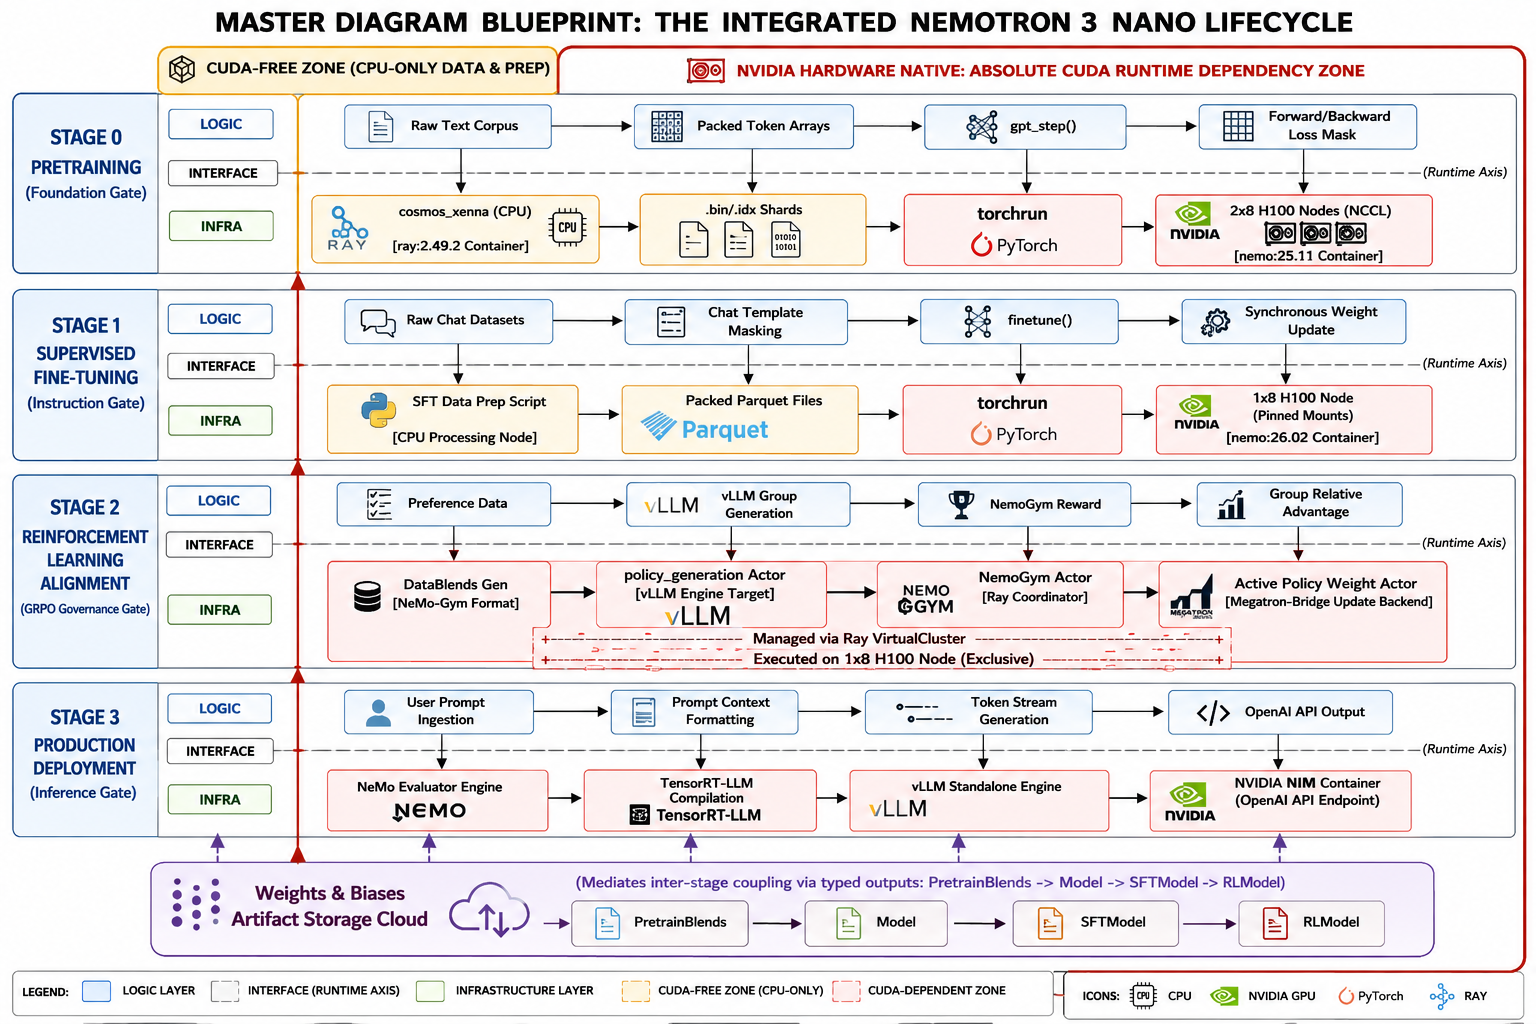
\includegraphics[width=0.85\textwidth]{images/figures/infra-dependecy-highlight.png}
    \caption{NVIDIA Infrastructure Dependency Diagram}
    \label{fig:NVIDIA Infrastructure Dependency Diagram}
\end{figure}



% ── 3.3.5 ────────────────────────────────────────────────────
\subsection{Experiment Tracking and Artifact Management}
\label{subsec:wandb-artifacts}

Weights \& Biases serves two distinct roles in the pipeline: experiment
tracking and artifact lineage management. W\&B is initialised in each
stage to capture training metrics, configuration snapshots, and
checkpoint logs, with several monkey-patches applied to ensure
compatibility with Megatron-Bridge. The pipeline also uses W\&B
artifacts as the inter-stage handoff mechanism, creating an unbroken
lineage graph from raw datasets to the final aligned model, as
documented in \tabref{artifact-lineage}.

\begin{table}[htbp]
  \centering
  \caption{W\&B artifact lineage across pipeline stages}
  \label{tab:artifact-lineage}
  \begin{tabularx}{\textwidth}{>{\hsize=0.7\hsize}L >{\hsize=1.0\hsize}L >{\hsize=1.0\hsize}L >{\hsize=1.3\hsize}L}
    \toprule
    \tableheader{Stage & Artifact In & Artifact Out & Type} \\
    \midrule
    Pretrain data prep
      & Raw datasets
      & \path{nano3-pretrain-data:latest}
      & \texttt{PretrainBlendsArtifact} \\
    \rowcolor{TableRowOdd}
    Pretraining
      & \path{nano3-pretrain-data:latest}
      & \path{nano3-pretrain-model:latest}
      & \texttt{ModelArtifact} \\
    SFT data prep
      & Raw chat datasets
      & \path{nano3-sft-data:latest}
      & \texttt{SFTDataArtifact} \\
    \rowcolor{TableRowOdd}
    SFT
      & \path{nano3-pretrain-model:latest} + \path{nano3-sft-data:latest}
      & \path{nano3-sft-model:latest}
      & \texttt{ModelArtifact} \\
    RL data prep
      & Raw preference datasets
      & \path{nano3-rl-data:latest}
      & \texttt{DataBlendsArtifact} \\
    \rowcolor{TableRowOdd}
    RL (GRPO)
      & \path{nano3-sft-model:latest} + \path{nano3-rl-data:latest}
      & \path{nano3-rl-model}
      & \texttt{ModelArtifact} \\
    \bottomrule
  \end{tabularx}
\end{table}
